\documentclass[12pt]{article}
\usepackage[T1]{fontenc}
\usepackage[utf8]{inputenc}
\usepackage[margin=1.2in]{geometry}
\usepackage{graphicx}
\usepackage{mathtools}
\usepackage{indentfirst}
\usepackage{float}
\usepackage{listings}
\usepackage{tabularx}
\usepackage{array}
\usepackage{wrapfig}
\usepackage{multirow}
\usepackage{graphicx} %Loading the package
\usepackage{verbatim}
\graphicspath{{../figs/}} %Setting the graphicspath

\usepackage[dvipsnames]{xcolor}

\usepackage{fancyvrb}

% redefine \VerbatimInput
\RecustomVerbatimCommand{\VerbatimInput}{VerbatimInput}%
{fontsize=\footnotesize,
 %
 frame=lines,  % top and bottom rule only
 framesep=2em, % separation between frame and text
 rulecolor=\color{Gray},
 %
 label=\fbox{\color{Black}scParams.txt},
 labelposition=topline,
 %
 commandchars=\|\(\), % escape character and argument delimiters for
                      % commands within the verbatim
 commentchar=*        % comment character
}

\usepackage{pdfpages} 

\title{AEM 4305 - SADC \\ 
MayFly Mission: \\
Attitude Dynamics} 
\author{By: Garrett Ailts}
\date{Mar 23 2020}

\begin{document}
\maketitle
\thispagestyle{empty}
\newpage

\section{Attitude Equations of Motion}
On the following pages are the hand calculations for the attitude equations of motion of the MayFly spacecraft. This includes a calculation of the spacecraft's moment of inertia matrix about the center of mass aligned with the principal axes. For now, we assume the spacecraft has a constant volumetric density \(\sigma\), which is calculated using the desired spacecraft wet mass and the volume of the spacecraft chassis (16U ISIS CubeSat at Max Dimensions). The hand calculations were used to write a MATLAB function, scMOI.m, which calculates the moment of inertia matrix w.r.t. to the spacecraft center of mass and aligned with the principal axes of inertia. This function can be viewed in the appendix.
\includepdf[pages=-]{Semester_Project/docs/SADC_PP3/pdf/SADC_PP3_P1}



%\VerbatimInput{Semester_Project/params/scParams.txt}
%\newpage

\section{Numerical Simulation of Attitude Dynamics}
A numerical simulation was conducted to propagate the spacecraft's attitude through time. The simulation is first done by storing the attitude using the quaternion representation. The simulation is then ran again using the DCM representation by storing all nine DCM parameters in the state vector. Both representations yielded identical results. 

\subsection{Simulation using the quaternion representation} 
The following outputs show the spacecrafts quaternion parameters, euler angles, quaternion constraint, angular velocity $\omega^{ba}_{b}$, and the rotational energy $T_{Bw/a}$ w.r.t. time. A picture of an attitude animation for the spacecraft is also included.

\begin{figure}[H]
\centering
    \includegraphics[width=0.8\textwidth]{Semester_Project/figs/quat_attitude_qAttType.png}
    \caption{Quaternion parameters \(\epsilon\) and \(\eta\) w.r.t. time}
\end{figure}
\begin{figure}[H]
\centering
    \includegraphics[width=0.8\textwidth]{Semester_Project/figs/euler_angles_qAttType.png}
    \caption{Euler angles in degrees for a 3-2-1 euler sequence w.r.t. time}
\end{figure}
\begin{figure}[H]
\centering
    \includegraphics[width=0.8\textwidth]{Semester_Project/figs/quatConstraint.png}
    \caption{Quaternion constraint value w.r.t. time}
\end{figure}
\begin{figure}[H]
\centering
    \includegraphics[width=0.8\textwidth]{Semester_Project/figs/angular_rates_qAttType.png}
    \caption{Angular rates in rad/s w.r.t. time}
\end{figure}
\begin{figure}[H]
\centering
    \includegraphics[width=0.8\textwidth]{Semester_Project/figs/sc_rot_energy_qAttType.png}
    \caption{Rotational energy and normalized rotational energy w.r.t. time}
\end{figure}
\begin{figure}[H]
\centering
    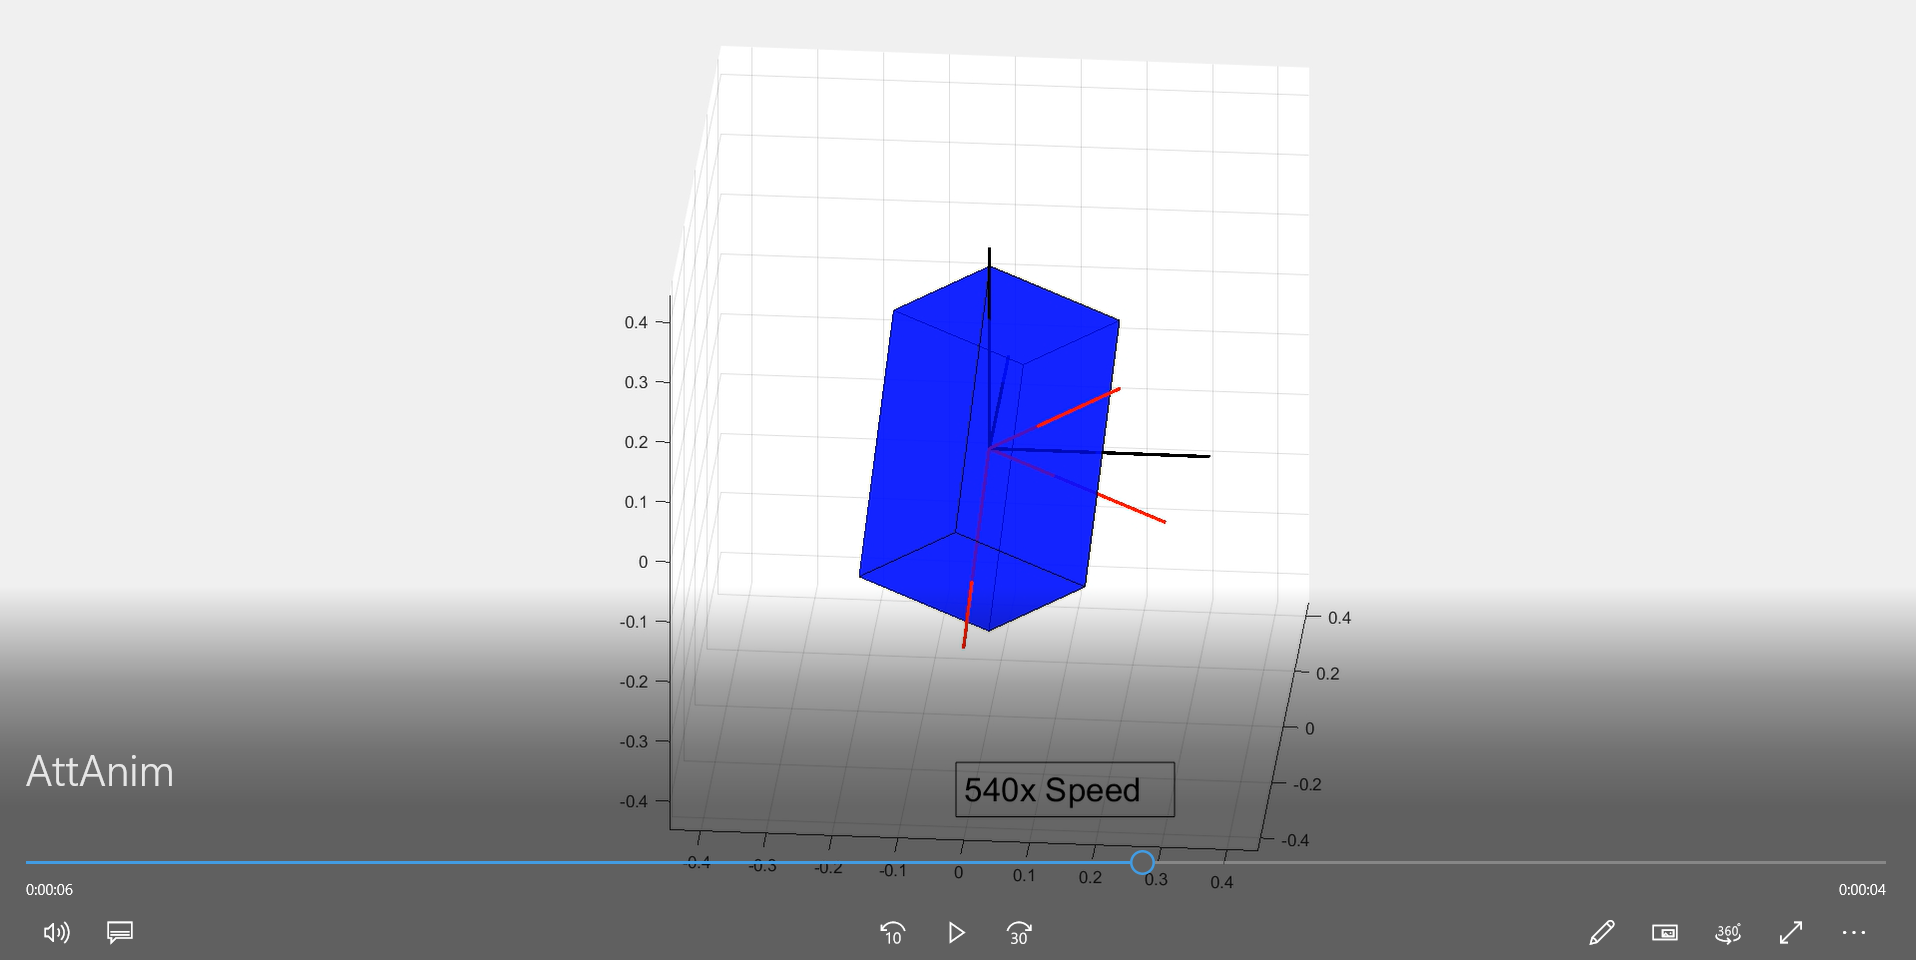
\includegraphics[width=0.8\textwidth]{Semester_Project/figs/AttitudeAnimPic.PNG}
    \caption{Snapshot of spacecraft attitude animation}
\end{figure}

\subsection{Simulation using the DCM representation}
All attitude simulation functions are written so they can function with both a quaternion and DCM attitude representation. Files and functions containing simulation parameters, the attitude simulation setup, the ODE's representing the dynamics, and post processing actions can be found in the appendix. The user simply needs to change the attitude type in the scParams.txt file.
\begin{figure}[H]
\centering
    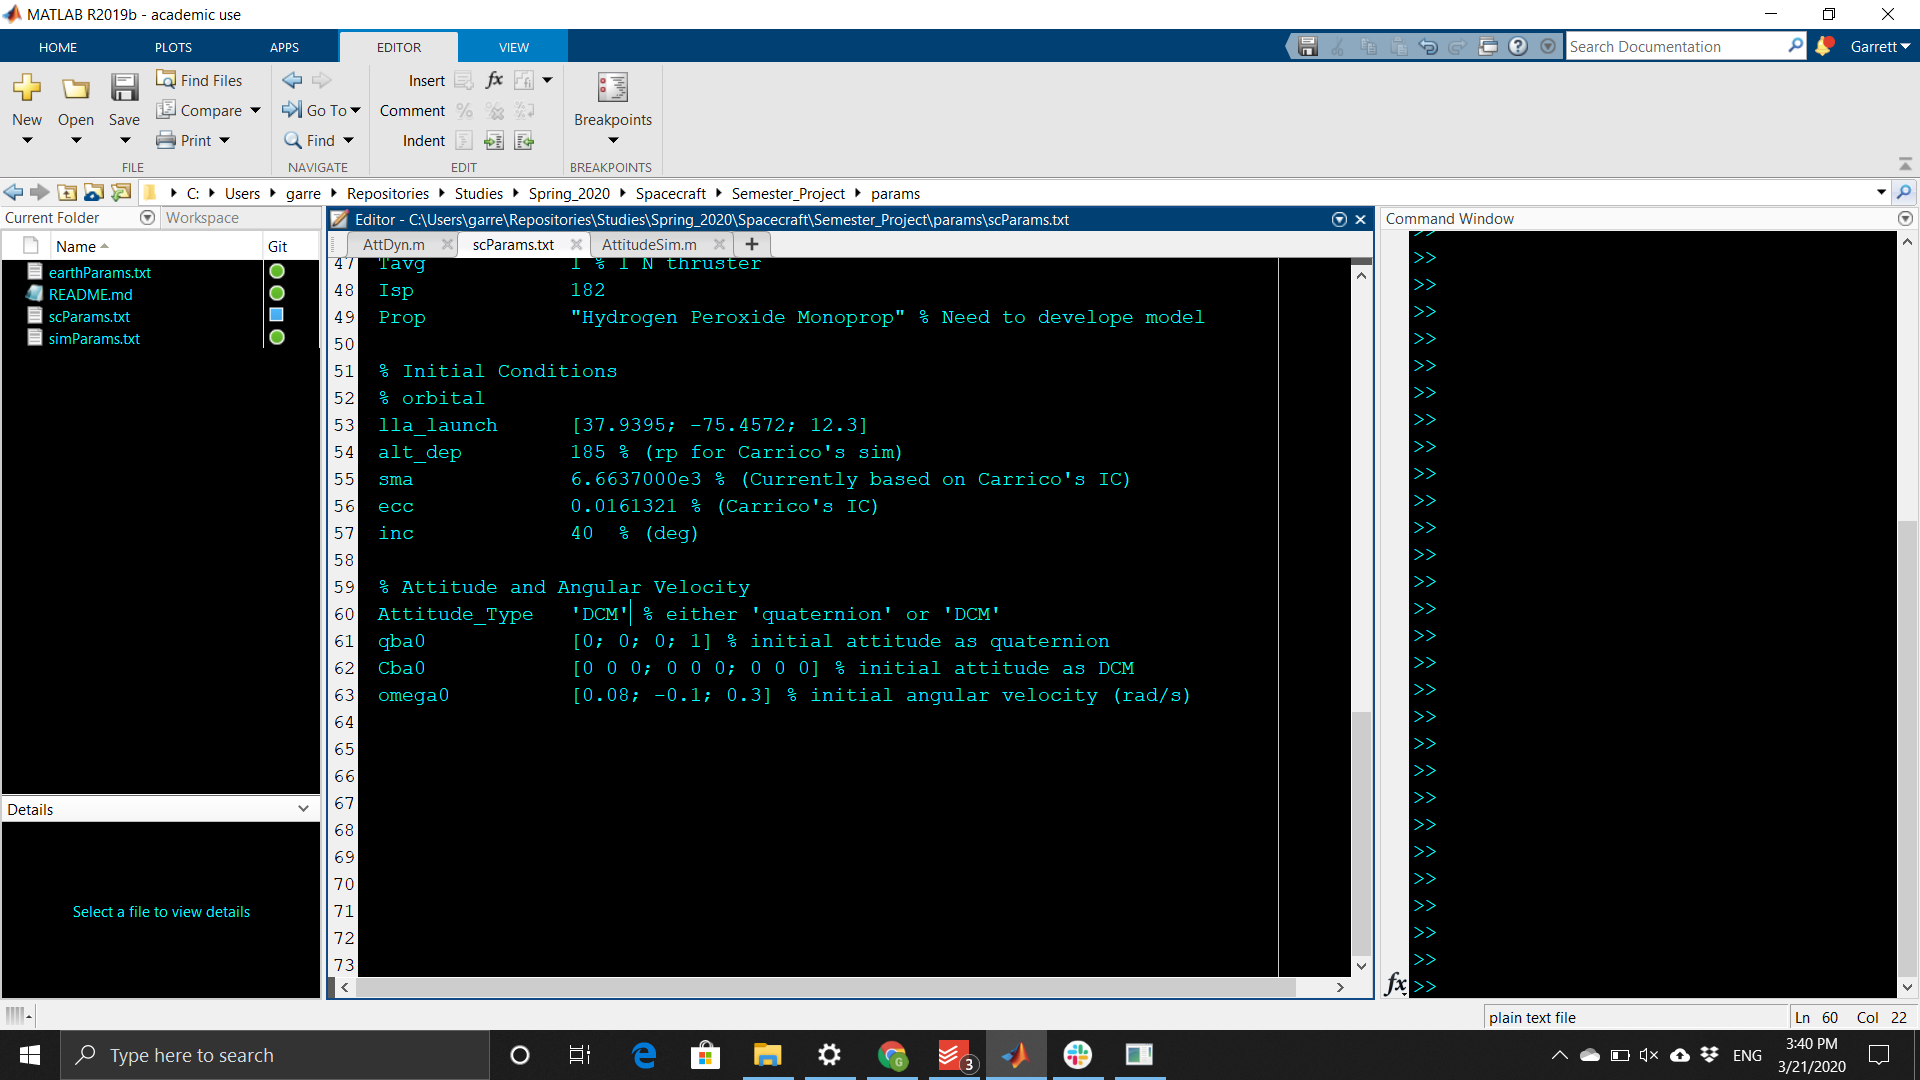
\includegraphics[width=1\textwidth]{Semester_Project/figs/Screenshot14.png}
    \caption{Example of configuring attitude type using the scParams.txt file in the params folder}
\end{figure}
After changing the attitude type, the simulation was ran again and the outputs were plotted. This time, the quaternion constraint is replaced by the normalized DCM contraint. Since the a valid DCM should always have a determinant of 1, we plot $det(C_{ba})-1$ to normalize the constraint to zero.


\begin{figure}[H]
\centering
    \includegraphics[width=0.8\textwidth]{Semester_Project/figs/euler_angles_DCM.png}
    \caption{Euler angles in degrees for a 3-2-1 euler sequence w.r.t. time extracted from the DCM}
\end{figure}
\begin{figure}[H]
\centering
    \includegraphics[width=0.8\textwidth]{Semester_Project/figs/constraint_DCM.png}
    \caption{DCM constraint value w.r.t. time}
\end{figure}
\begin{figure}[H]
\centering
    \includegraphics[width=0.8\textwidth]{Semester_Project/figs/angular_rates_qAttType.png}
    \caption{Angular rates in rad/s w.r.t. time}
\end{figure}
\begin{figure}[H]
\centering
    \includegraphics[width=0.8\textwidth]{Semester_Project/figs/sc_rot_energy_DCM.png}
    \caption{Rotational Energy and normalized rotational energy w.r.t time}
\end{figure}


\section{Appendix}
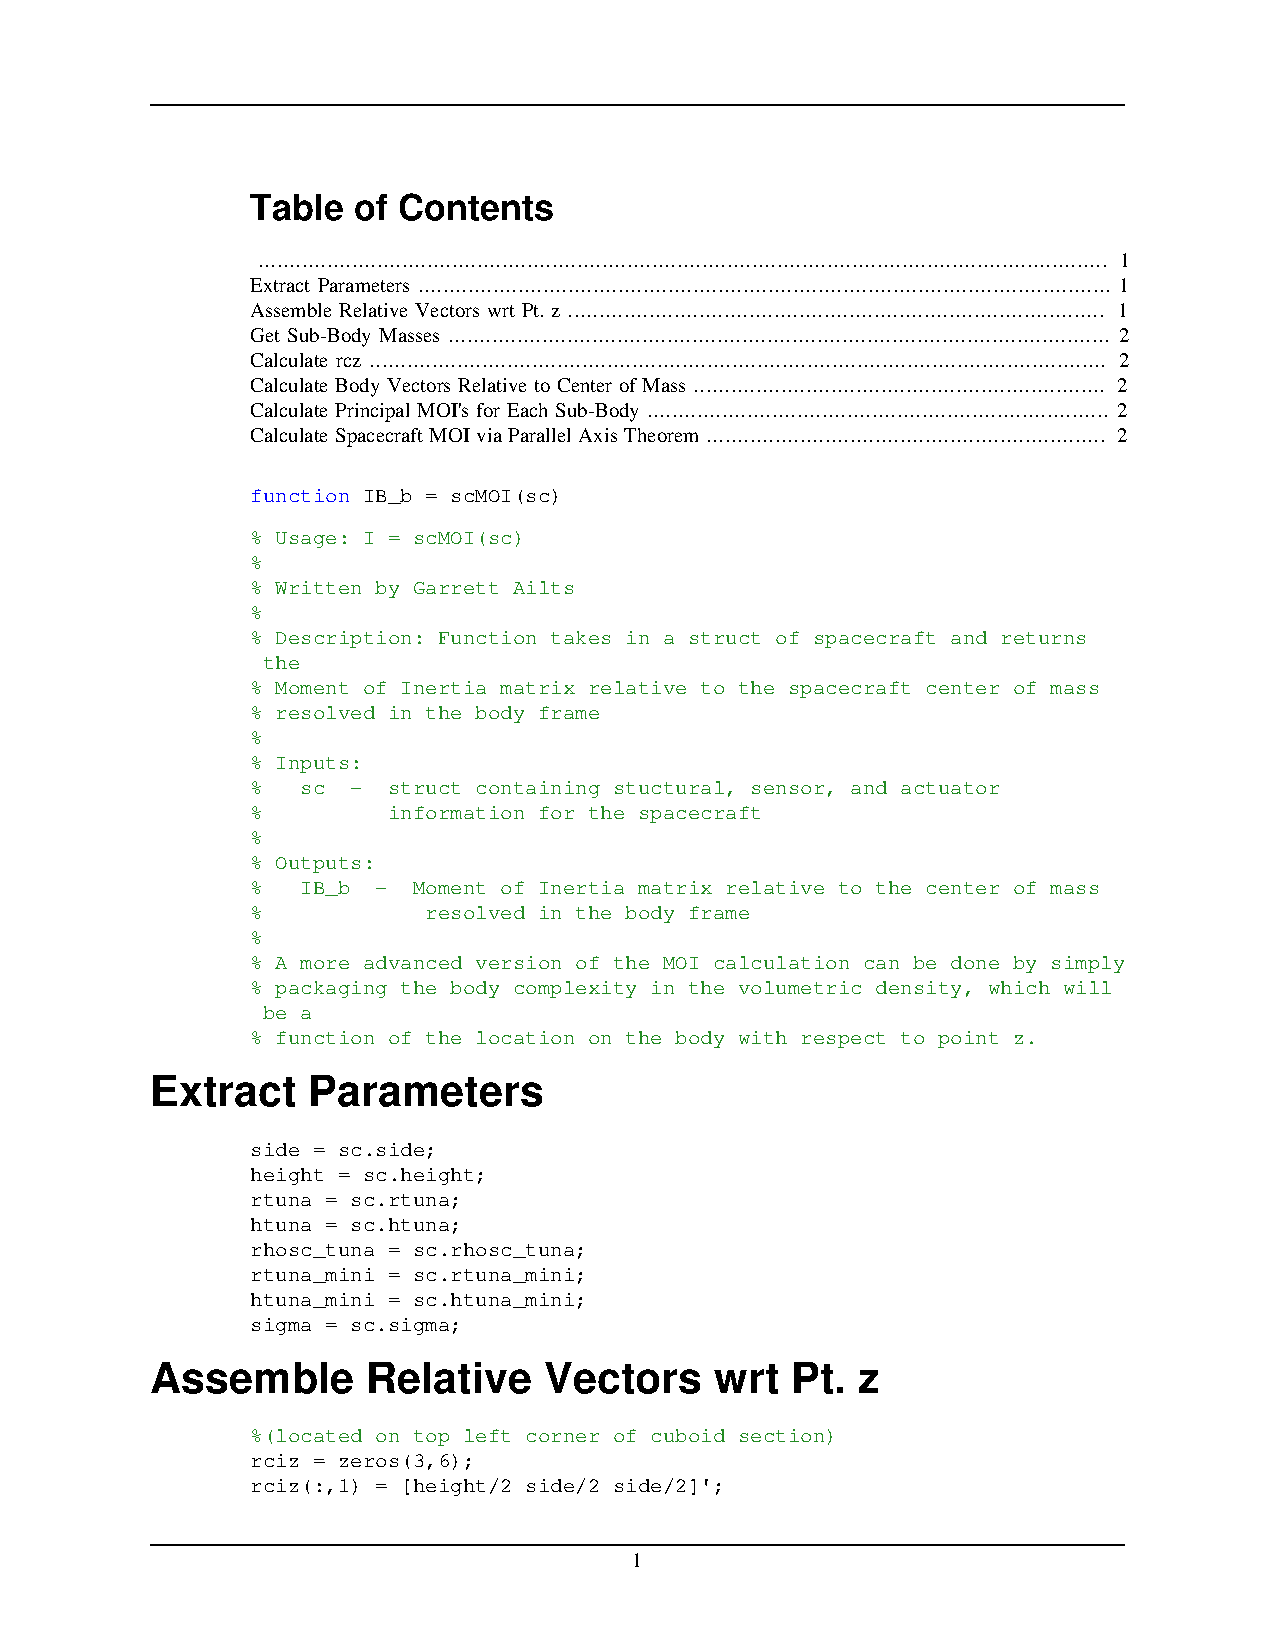
\includepdf[pages=-]{Semester_Project/docs/SADC_PP3/pdf/scMOI}
\VerbatimInput{Semester_Project/params/scParams.txt}
The values in this file are loaded into a parameter struct using the function loadParams.m, which was shown in the previous project.
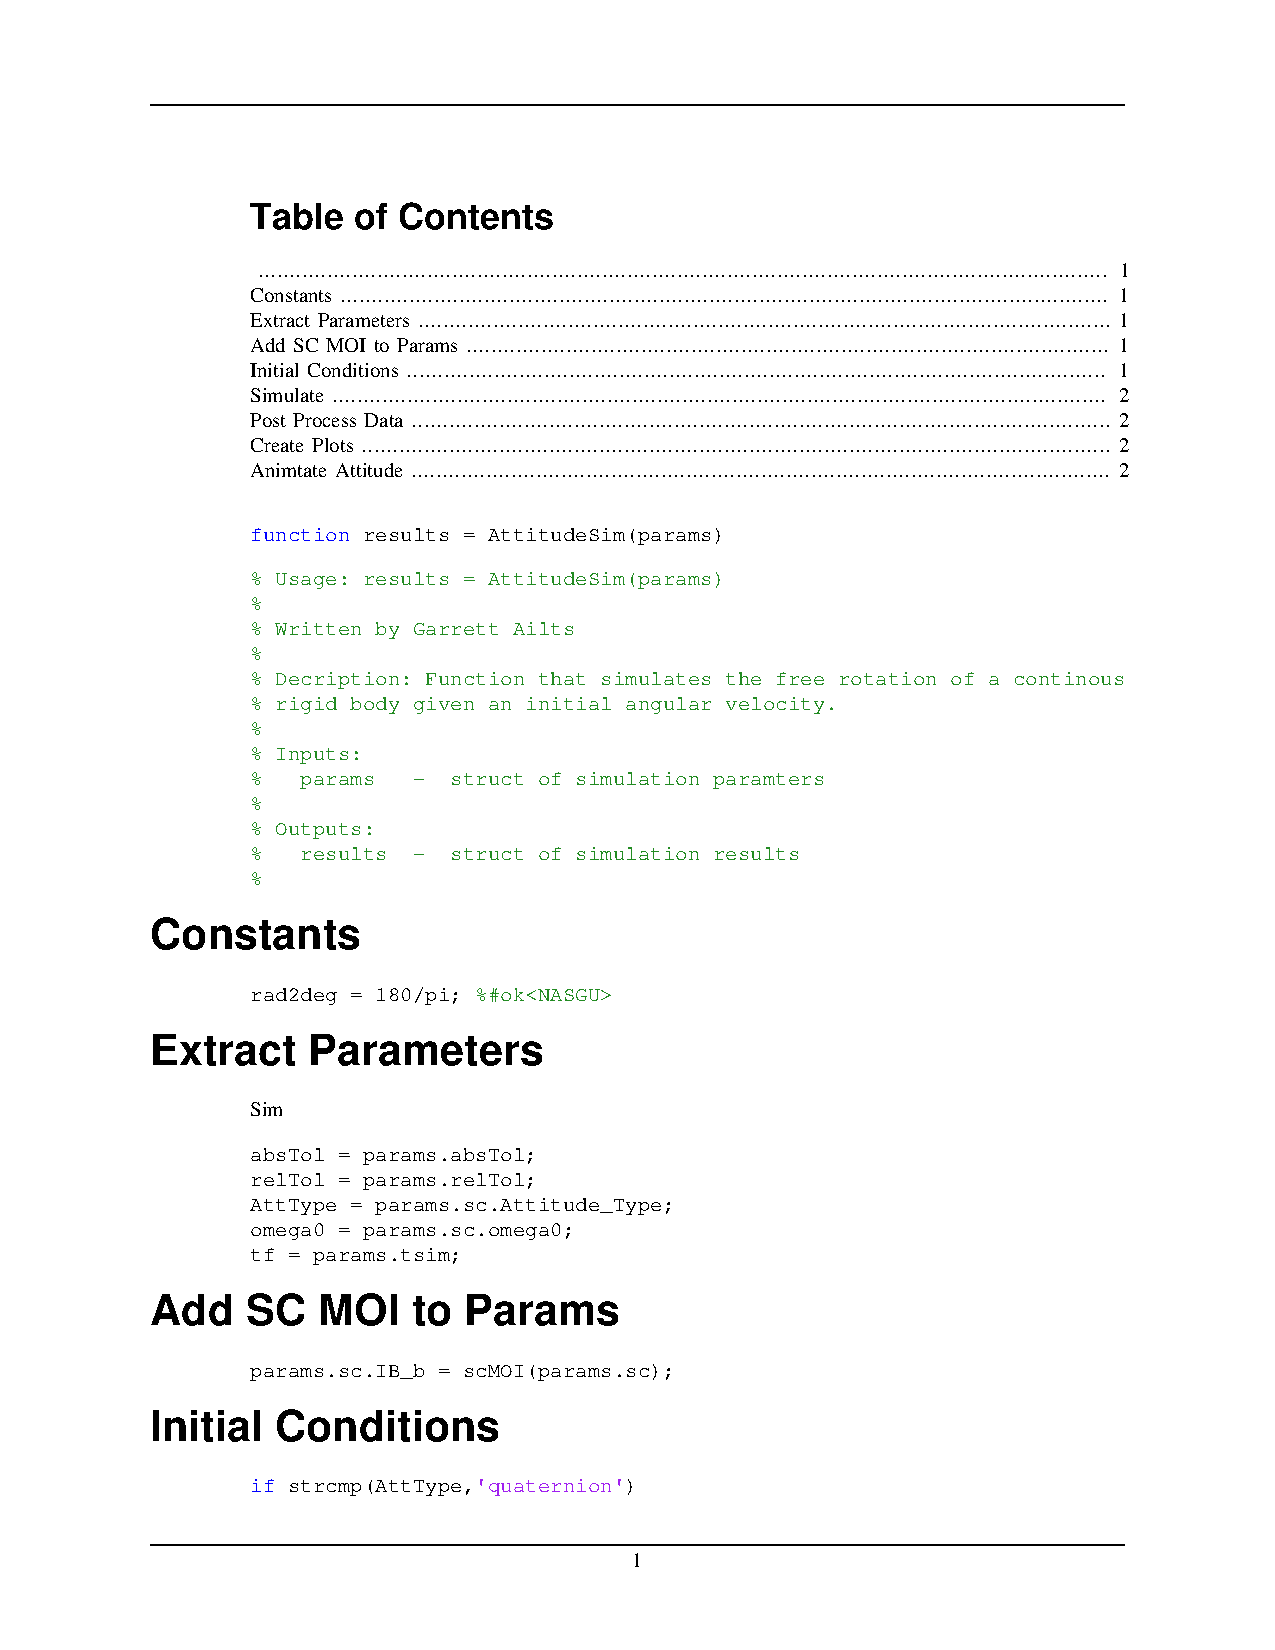
\includepdf[pages=-]{Semester_Project/docs/SADC_PP3/pdf/AttitudeSim}
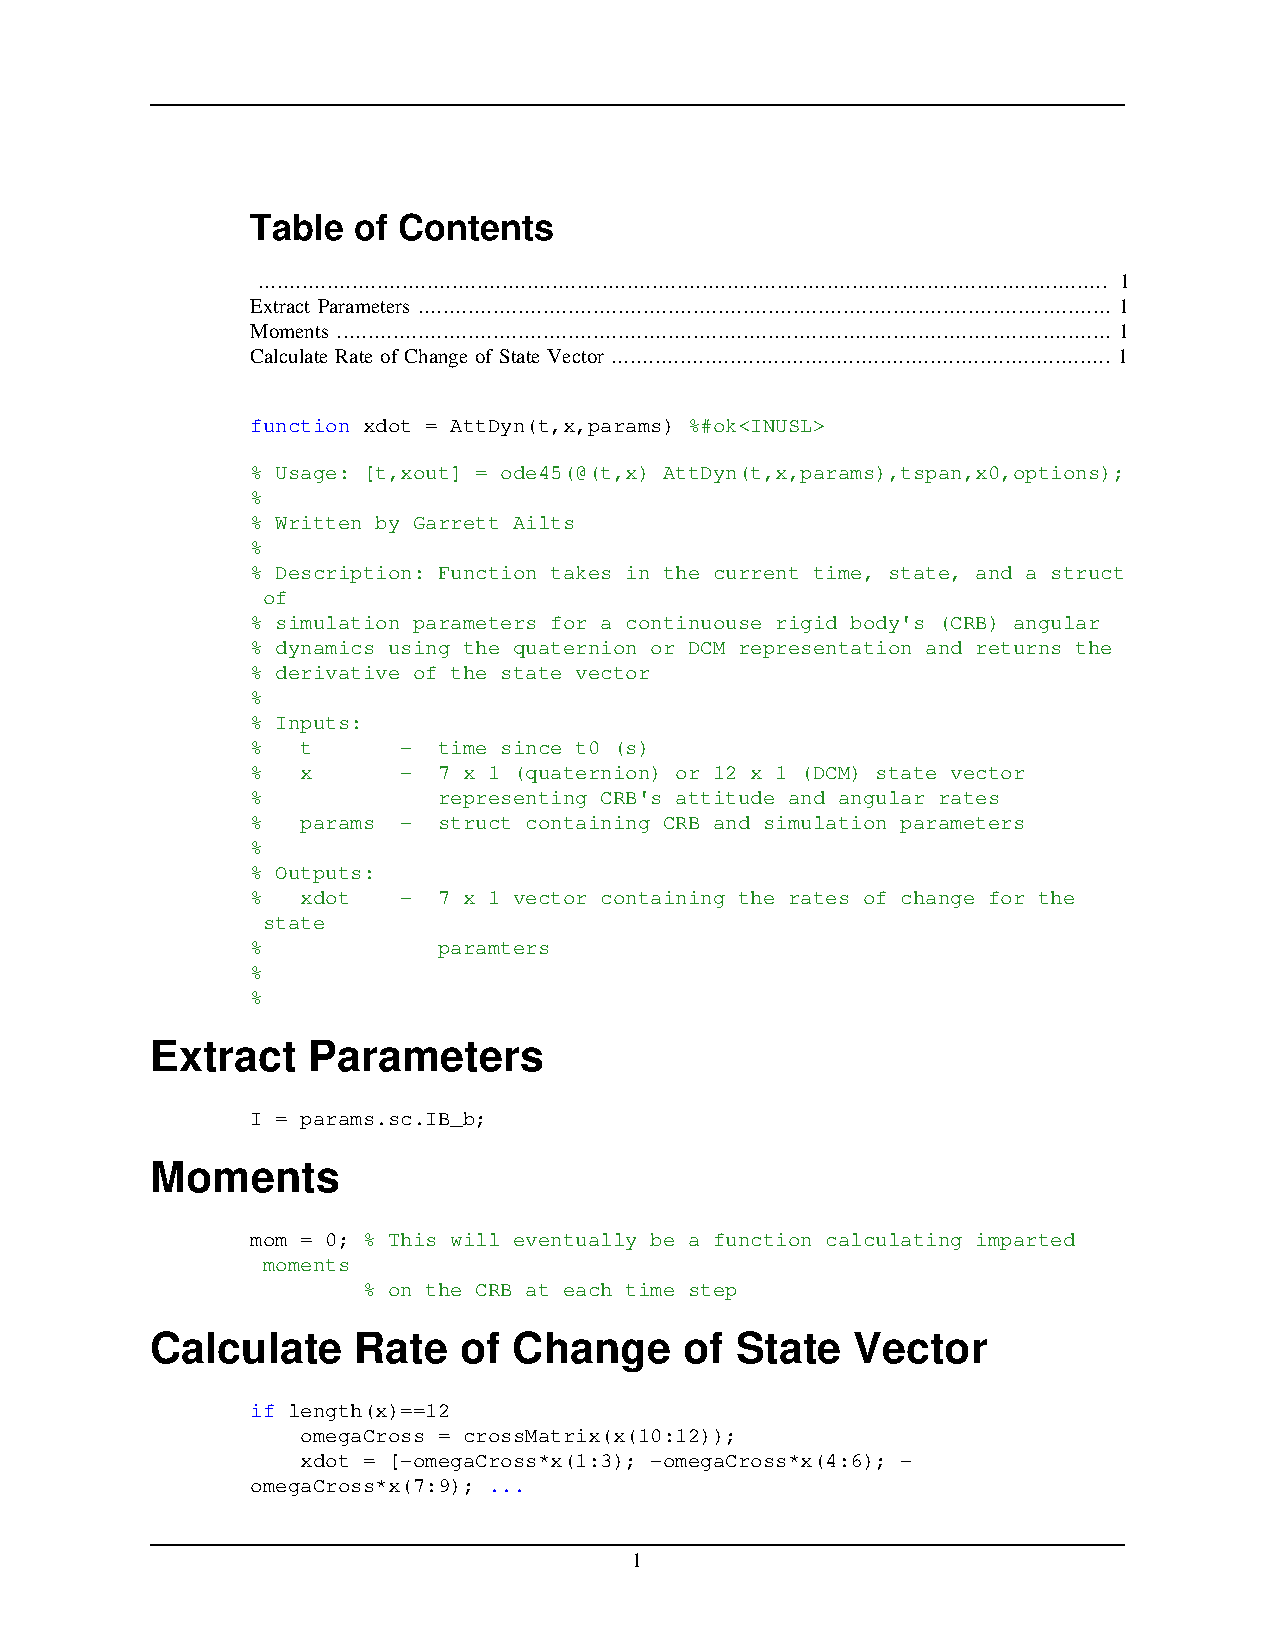
\includepdf[pages=-]{Semester_Project/docs/SADC_PP3/pdf/AttDyn}
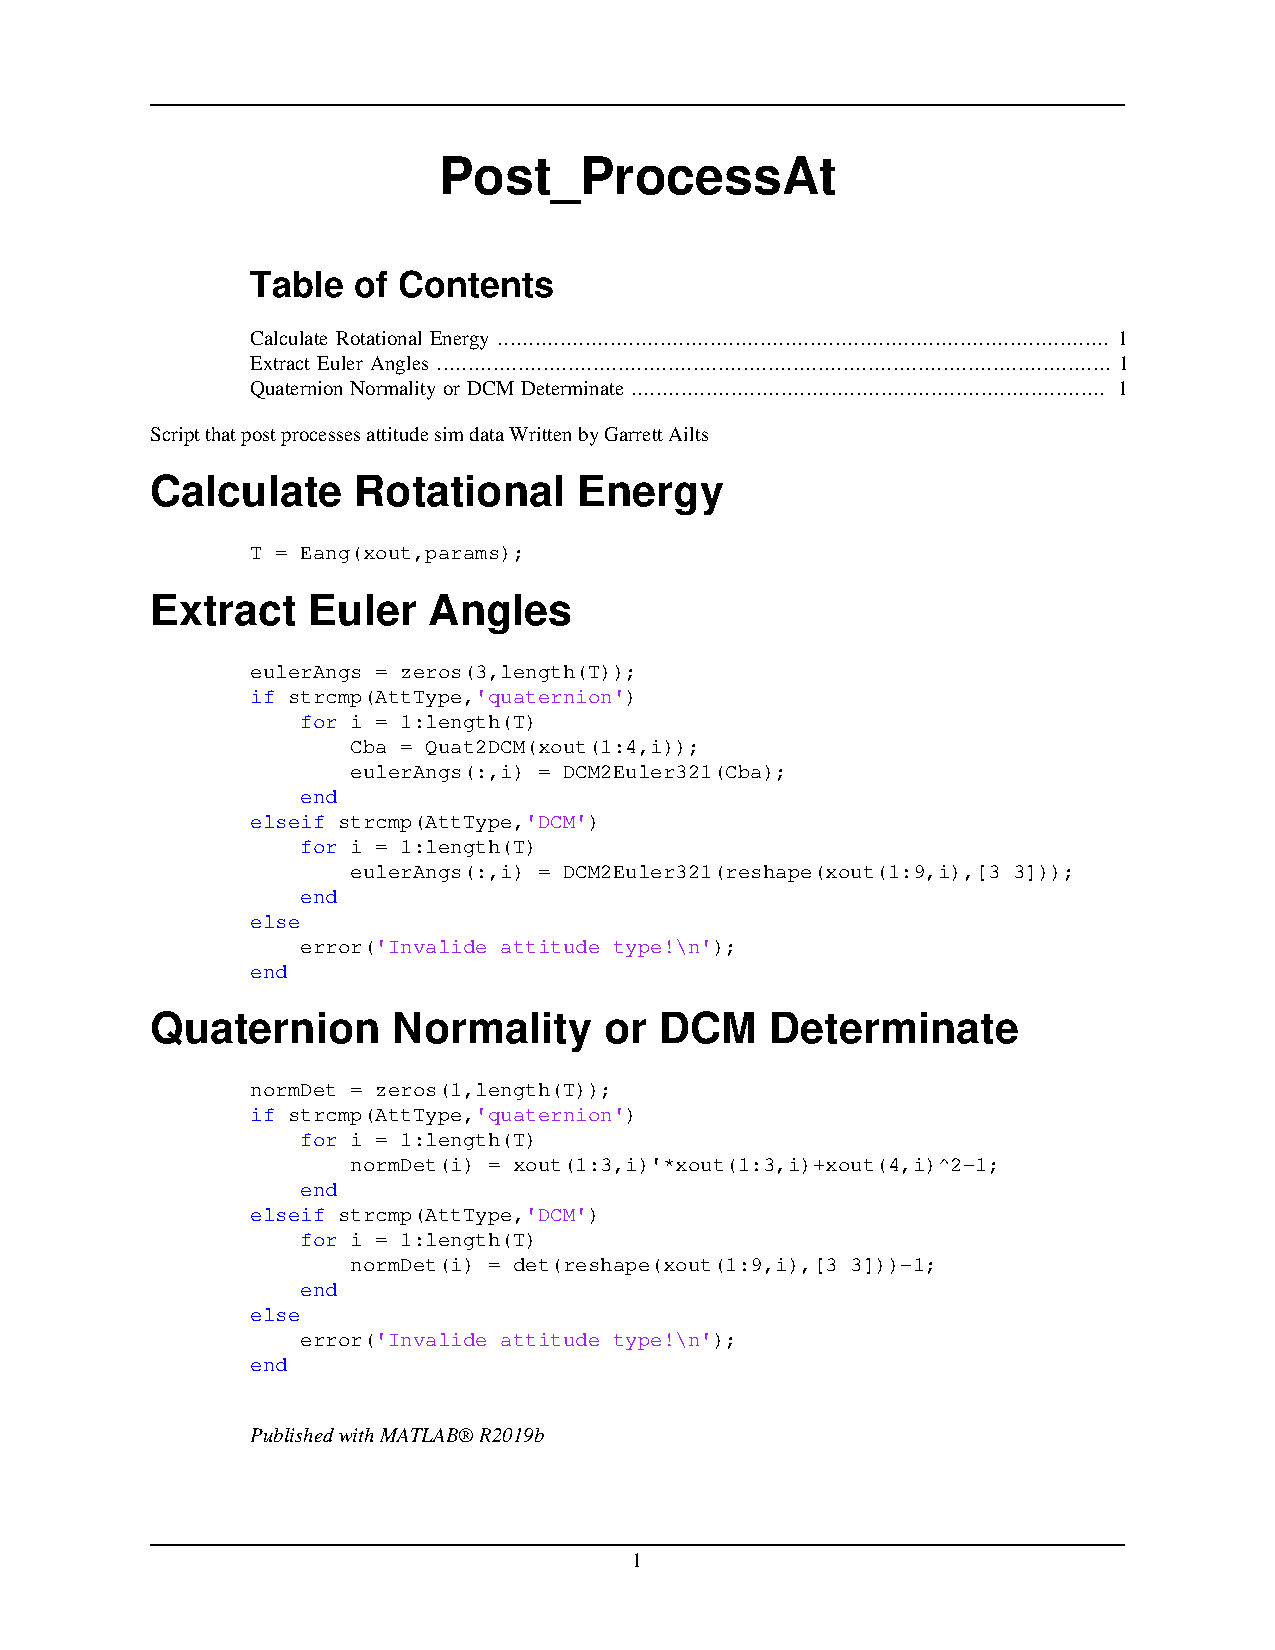
\includepdf[pages=-]{Semester_Project/docs/SADC_PP3/pdf/Post_ProcessAt}
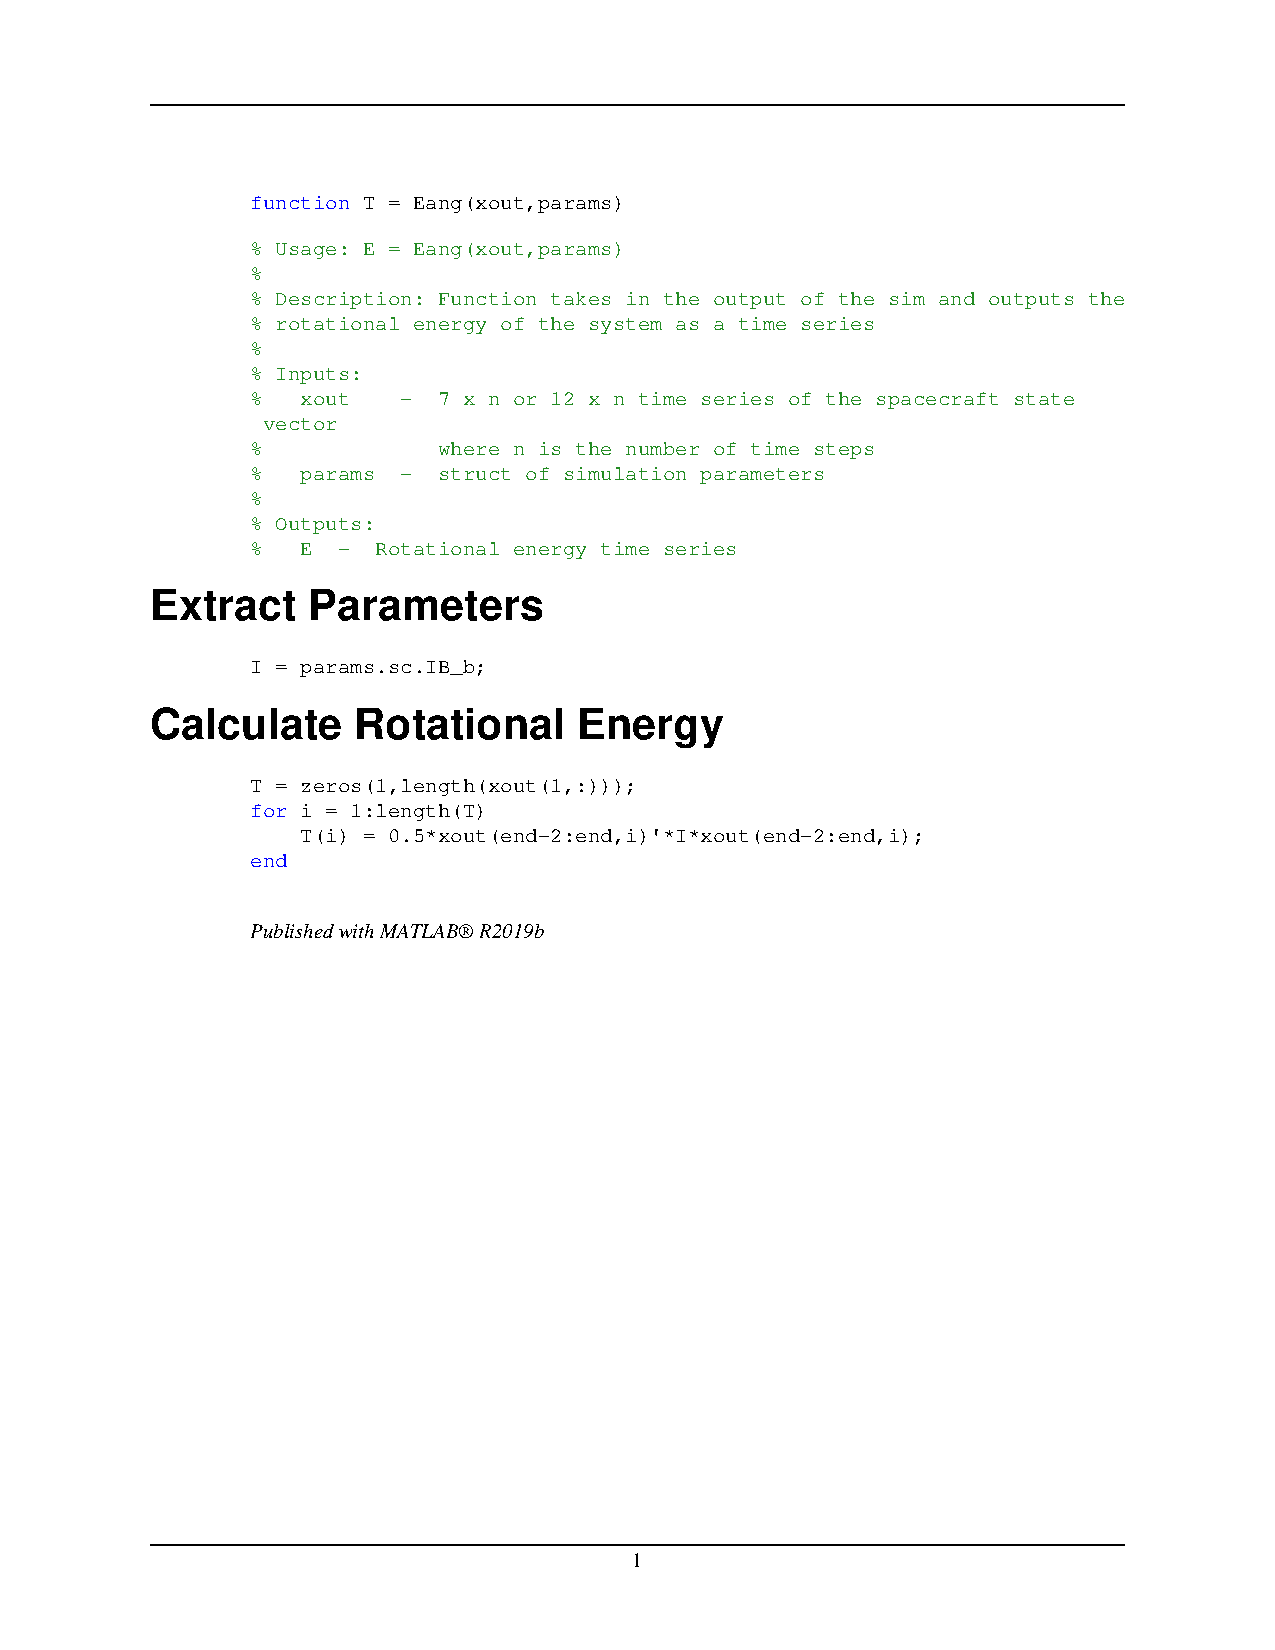
\includepdf[pages=-]{Semester_Project/docs/SADC_PP3/pdf/Eang}



\end{document}
